 
\chapter{$Ca^{2+}$ signalling models for fertilisation}
There are many models of $Ca^{2+}$ signalling available, including {those} derived by \citeA{Theodoridou2013} and \citeA{hofer}. \citeA{Sanders2018} is also based on these models. In the model by \citeA{Theodoridou2013} there are three equations for cytosolic $Ca^{2+}$ concentration, represented by $c$, $Ca^{2+}$ concentration in the ER, represented by $c_e$, and cytosolic $IP_3$ concentration, represented by $p$. Since $c_e$ plays more of a passive role \shortcite{Sanders2018,wakai}, one should be able to replace it with a constant, with the system continuing to oscillate. In many models the $IP_3R$ dynamics have been considered in the modelling of the flux of $Ca^{2+}$ from the ER into the cytosol. However, these can be eliminated, or disregarded, in many instances with the systems still producing oscillations. For the model by \citeA{Sanders2018} upon numerical experimentation, we found that oscillations are lost when $c_e$ is taken out.  {This can be seen in Figure \ref{sandersfig}.} This implies a dependence on ER store refilling, rather than $IP_3R$ dynamics. By considering a gating model instead, for example the model by \citeA{atri}, we have a two--variable model that does not consider $Ca^{2+}$ in the ER as a dynamic variable. Regardless of this, it is still necessary that the model incorporates the correct $IP_3R$ dynamics. The most recent data for $IP_3R$ dynamics are discussed in Chapter 3, where we review the paper by \citeA{Mak1998}. 
\begin{figure}[!htb]
\centering
\minipage{0.6\textwidth}
  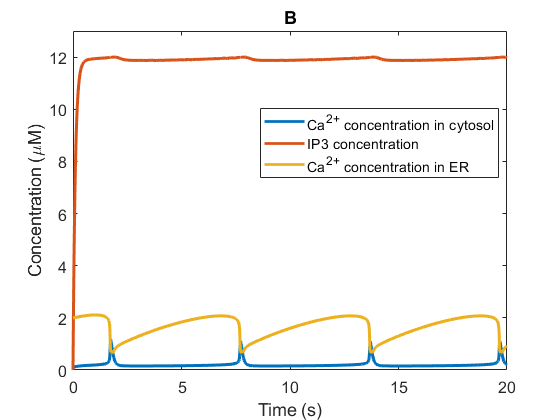
\includegraphics[width=\linewidth]{Chapters/2_Ca2+_Models/extras/oscillations.png}
\endminipage\hfill\\
\minipage{0.6\textwidth}
  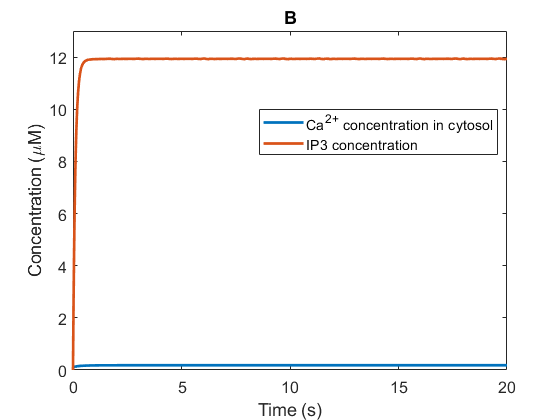
\includegraphics[width=\linewidth]{Chapters/2_Ca2+_Models/extras/no_oscillations.png}
\endminipage\hfill
\caption{{$Ca^{2+}$ oscillations arising as solutions to the \shortcite{Sanders2018} model. (\textbf{A}) Cytosolic $Ca^{2+}$, $IP_3$, and $Ca^{2+}$ in the ER oscillating. (\textbf{B}) A non oscillatory system of cytosolic $Ca^{2+}$ and $IP_3$, with the equation for $Ca^{2+}$ in the ER having been taken out. This implies that oscillations depend on the ER store refilling.} \textit{Software:} MATLAB.}\label{sandersfig}
\end{figure}

\begin{figure}[h!!!t!!!b!!!p]
  \centering
  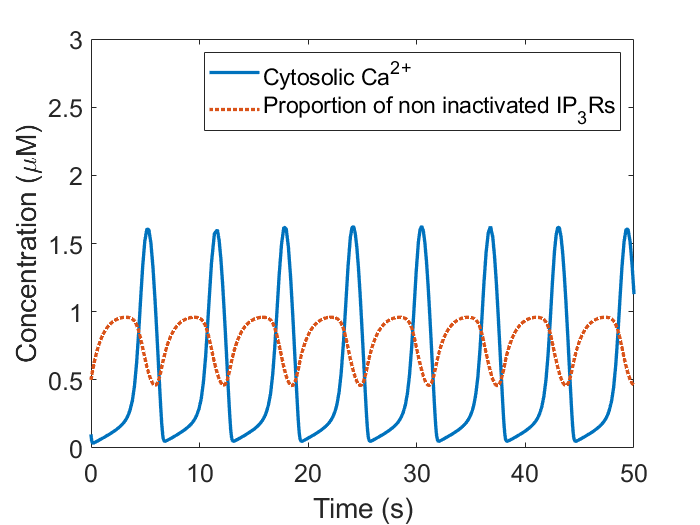
\includegraphics[width=0.6\linewidth]{Chapters/2_Ca2+_Models/extras/orginalatrimu1.png}
  \caption{$Ca^{2+}$ oscillations as solutions to the Atri Model, (\ref{origatri1stnondim}), (\ref{origatri2ndnondim}), with $\mu(p)=0.3$ (within oscillatory range). Parameter values are shown in Table \ref{origatriparam}. Initial values of $0.1\mu M$ and $0.5$ were taken for $c$ and $n$ respectively. Oscillations over time of $50$ seconds. \textit{Software:} MATLAB.}\label{figorigatri}
\end{figure}

Taking the recent models mentioned as our starting point we resolve issues and correct the dependence on the $IP_3R$ dynamics. We should avoid oscillations that depend on the ER store depletion. We are motivated to go back to basics and identify {how to incorporate} the open probability equation by \citeA{Mak1998}. We have briefly mentioned some well-established models for $Ca^{2+}$ signalling in our introduction. Here we revisit these models in a detailed manner and decide which model would be suitable to incorporate the correct $IP_3R$ dynamics into.

Below we study two key deterministic models for $Ca^{2+}$ oscillations. We explore how they work, especially what drives the $Ca^{2+}$ oscillations, and their biological representation. We begin by looking at model by \citeA{atri} and the model by \citeA{lirinzel}.

\section{The Atri et al. model}

The first model we review was developed by \citeA{atri}. It is the first deterministic $Ca^{2+}$ model for the Xenopus oocyte. This model displays a fairly realistic representation of $Ca^{2+}$ signals that occur during fertilisation. The model is based on experimental evidence that the $IP_3R$ is regulated by the cytosolic $Ca^{2+}$ level in a biphasic manner \shortcite{finchetal}. It is apparent in the experiments that $Ca^{2+}$ release is inhibited by both low and high levels of cytosolic $Ca^{2+}$, and encouraged by intermediate levels of cytosolic $Ca^{2+}$. The inactivation of the $IP_3R$ is a slower process than the activation \shortcite{finchetal}. The model produces $Ca^{2+}$ oscillations and travelling waves in the Xenopus Laevis oocyte with $IP_3$ concentration at a constant level.

The model consists of two ODEs, \eqref{origatri1st} and \eqref{origatri2nd}, where $c$ represents cytosolic $Ca^{2+}$ concentration (in $\mu M$) and $n$ represents the  proportion of non inactivated $IP_3$ 
receptors. The ODEs are:
\begin{align}
    \frac{dc}{dt}&= J_{channel}-J_{pump}+J_{leakage},\label{origatri1st}\\
    \tau_n\frac{dn}{dt}&=\frac{K_{inh}^2}{K_{inh}^2+c^2}-n.\label{origatri2nd}
\end{align}
The fluxes above are given by
\begin{align}\nonumber
    J_{channel}&=k_{flux}n\left(\frac{p+\mu_0K_{IP_3}}{K_{IP_3}+p}\right)\left(\frac{K_{act}b+c}{K_{act}+c}\right),\nonumber\\
    J_{pump}&=\frac{V_e c}{K_e+c},\nonumber\\
    J_{leakage}&=\delta.\nonumber
\end{align}
The $Ca^{2+}$ flux from the ER through the $IP_3R$ into the cell cytosol is represented by $J_{channel}$. The $Ca^{2+}$ flux by SERCA pumps from the cytosol to the cell's ER is represented by $J_{pump}$. {The small flux of $Ca^{2+}$ leaking out of the ER is represented by $J_{leakage}$}. Parameter values and biological descriptions are given in Table \ref{origatriparam}.

\subsection{Model assumptions}

\subsubsection*{The single channel model}
A few assumptions are made about the $IP_3R$ in the Appendix of \citeA{atri}. These are:
\begin{itemize}
    \item The $IP_3R$ consists of three independent binding sites.
    \item A single molecule of $IP_3$ binds to the $IP_3$ activation site (site 1). A single molecule of $Ca^{2+}$ binds to the $Ca^{2+}$ activation site (site 2), and two molecules of $Ca^{2+}$ bind to the ${Ca^{2+}}$ inhibitory site (site 3).
    \item Activation of sites 1 and 2, and inactivation of site 3 together permits $Ca^{2+}$ to pass through the $IP_3R$. Hence $Ca^{2+}$ is involved in both positive and negative feedback.
    \item When $Ca^{2+}$ and ${IP_3}$ levels are zero, basal flux through the $IP_3R$ is still assumed as there is still a nonzero probability of activation of sites 1 and 2.
    \item The number of open channels is responsible for the total flux of $Ca^{2+}$ from the ER to the cytosol. 
\end{itemize}

In $J_{channel}$ there are three terms multiplying each other, $p_1$, $p_2$, and $p_3$, which give the probability that a single channel is open. $p_1$ and $p_2$ represent the probabilities that sites 1 and 2 are activated, respectively. The probability that $Ca^{2+}$ is not bound to site 3 (inactivation site) is represented by $p_3$. We can, therefore, say that the total steady-state $Ca^{2+}$ flux through $IP_3R$ is given by the following:
\begin{equation}
    I_T=Nip_1p_2p_3,\nonumber
\end{equation}
where $i$ is the $Ca^{2+}$ current through a single open $IP_3R$ and $N$ is the total number of $IP_3R$.

In this paper it is assumed that the volume of a channel, $V$, is constant. {By this assumption, we can convert the $Ca^{2+}$ current to an impact of the flux on the concentration in the cytosol, given by $J_{channel}$:}
\begin{equation}
J_{channel}=\frac{Nip_1p_2p_3}{2FV},\label{converted}
\end{equation}
where $F$ represents Faraday's constant. {$J_{channel}$ is the $Ca^{2+}$ flux through the ER into the cytosol and has units $\mu Ms^{-1}$. It is directly proportional to the number of $IP_3R$ on the ER, $N$. The units of $F$ are $CM^{-1}$ and the units of $i$ are $\mu Cs^{-1}$. $N$ is dimenionless and $V$ has units of volume. $p_1$, $p_2$, and $p_3$ are true fluxes, in number of molecules per channel per second.}  To get to the final form of $J_{channel}$, let $k_{flux}=Ni/2FV$. Each of $p_1$, $p_2$, and $p_3$ are modelled as functions of $Ca^{2+}$ and ${IP_3}$, as labelled below. Note that we refer to $p_1$ as a function $\mu(p)$.

At steady state,
\begin{equation}
J_{channel}=k_{flux}\underbrace{\left({\frac{p+\mu_0K_{IP_3}}{K_{IP_3}+p}}\right)}_{p_1=\mu(p)}\underbrace{\left(\frac{K_{act}b+c}{K_{act}+c}\right)}_{=p_2}\underbrace{\left(\frac{K_{inh}^2}{K_{inh}^2+c^2}\right)}_{=p_3}.\label{atristeadystate}
\end{equation}
{It is an assumption of the Atri model that the expression for $J_{channel}$ valid at steady state also holds for the temporarily evolving system and this allows us to write ODEs \eqref{origatri1st} and \eqref{origatri2nd}. It is not our intention in this work to question this assumption.}

In this thesis, we aim to derive a more accurate model for $Ca^{2+}$ signalling at fertilisation. An area to focus and improve is the incorporation of $IP_3R$ dynamics. {The Atri model uses data \shortcite{parysetal} that inaccurately capture how the $IP_3R$ dynamics depend on $[Ca^{2+}]$ and $[IP_3]$ during fertilisation. We now have more accurate data for this from \shortciteA{Mak1998}.} It is therefore necessary to look closely at the components $p_1$, $p_2$, and $p_3$, as they synthesize the open probability of the $IP_3R$.

We can begin by studying $p_1$ further. As labelled above, we have called this $\mu(p)$. {$\mu_p$ is the probability that a single molecule of $IP_3$ binds to site 1. From experimental data, this probability is given to be $\mu_0=0.567$ when $IP_3=0$. The model then assumes that for non-zero $[IP3]$ the probability increases according to a Hill function and saturates at the value $1$. This Hill function is not fitted experimentally.} The half-maximal activation constant for $IP_3$ is given by $K_{IP_3}$. Note that $\mu_0+\mu_1=1$, where $\mu_1$ is the proportion of $IP_3R$ that are not activated at $IP_3=0 \mu M$.

Next, $p_2$ is the probability that $Ca^{2+}$ binds to activation site 2. The half-activation constant (the proportion of $IP_3R$ that are activated by the binding of $Ca^{2+}$) here is given by $K_{act}$. The parameter $b$ is the proportion of $IP_3R$ that have site 2 activated in the absence of bound $Ca^{2+}$ and represents a basal current through the $IP_3R$. 

Finally, the last component accountable for the opening of the $IP_3R$ is $p_3$, which represents the probability that $Ca^{2+}$ is not bound to inhibitory site 3. The half-maximal inactivation constant is $K_{inh}$. In $p_3$, the Hill coefficient of 2 shows that this is a more cooperative process than the binding in sites 1 and 2 (in $p_1$ and $p_2$), according to the data collected. According to the experiments, when $Ca^{2+}$ increases quickly, the $IP_3R$ is activated quickly and is deactivated very slowly. This is why site 3 takes a while to reach its steady state, hence the constant time scale, $\tau_n=2s$ in equation \eqref{origatri2nd}. This is despite the fact that sites 1 and 2 obtain a fast equilibrium with $IP_3$ and $Ca^{2+}$. 

The parameters $b$, $K_{act}$, and $K_{inh}$ for this model were all chosen by fitting to the experimental data in \citeA{parysetal}. We will revisit the functions of $p_1$, $p_2$, and $p_3$ and the way the open probability is modelled in Chapter 4, where we derive a new model.

\subsubsection*{Dynamic behaviour of the $\mathbf{IP_3R}$}
Equation \eqref{atristeadystate} represents the steady flux through the $IP_3R$ for fixed $Ca^{2+}$, but we must note that the channel reacts in a certain manner to a varying cytosolic $Ca^{2+}$ level. It is evident from the data in \citeA{finchetal} that when the cytosolic $Ca^{2+}$ concentration rapidly increases, the $IP_3R$ activates quickly and deactivates at a slower pace. This motivates the assumption that the binding of sites 1 and 2 quickly reach an equilibrium with $IP_3$ and cytosolic $Ca^{2+}$, while site 3 reaches its steady state proportional to the time constant $\tau_n$. We obtain equation \eqref{origatri1st} when we write $p_3$ as $n$ for notational convenience in equation \eqref{atristeadystate}. Note that the way in which the $IP_3R$ has been modelled shares similarities with the modelling of the $IP_3R$ subunits in the \citeA{hodgkinhuxley} model of electrical impulse propagation in the nerve axon, hence the Atri model is considered a gating model.  {In both models, constants were chosen in order to reproduce a specific steady-state curve for the open probability of the specific channels. In the Hodgkin-Huxley equations, these are the sodium and potassium channels as a function of voltage, and in the Atri model, this is the $IP_3R$ as a function of $Ca^{2+}$ and $IP_3$. The variable $n$, for the proportion of non inactivated $IP_3R$,
is directly analogous to the inactivation variable $h$ in the
Hodgkin-Huxley equations. Time constants in the equations for $n$ and $h$ account for the delay in activation and inactivation after changes in $[Ca^{2+}]$ and voltage, respectively.}

The modelling of the $IP_3R$ in the Atri model is very similar to other models, particularly the model by \citeA{deyoungkeizer}. Both of the models show similar results. Both feature a separation of time scales of $Ca^{2+}$-dependent activation and inactivation of the $IP_3R$, where activation takes places faster than inactivation \cite{finchetal}.

We have discussed which parts of this model represent $Ca^{2+}$ flux through to the cytosol (in $J_{channel}$), and that $J_{pump}$ represents the SERCA pumps back into the ER. The latter is given by the {Michaelis-Menten function}. It is acknowledged in the paper by \citeA{atri} that incorporation of more detail in this term would be beneficial to the model when more experimental evidence is available. The model is not driven by ER $Ca^{2+}$ depletion as the ER concentration is assumed to remain constant (and high). This emphasizes the importance of the role that the $IP_3R$ dynamics and the $IP_3$ concentration play in  facilitating the cytosolic $Ca^{2+}$ oscillations. That being said, as we see later, the $IP_3R$ dynamics that are used in the Atri model are based on outdated experimental data. A replacement in the dynamics is therefore due. We will do this in Chapter 3 with updated data from \citeA{Mak1998}.

\subsection{Non-dimensionalisation of the Atri et al. model}
We non-dimensionalise equations \eqref{origatri1st} and \eqref{origatri2nd} by substituting in $c=K_{act}\bar{c}$, $t=\tau_n\bar{t}$, and $n=\bar{n}$, as in \shortciteA{kaouri}. The process of non-dimensionalisation is discussed in \shortciteA{murray1989}. Dropping the bars for notational purposes, we get the following:
\begin{align}
    \frac{dc}{dt}&=\mu(p)K_1n\left(\frac{b+c}{1+c}\right)-\frac{Vc}{K+c},\label{origatri1stnondim}\\
    \frac{dn}{dt}&=\frac{K_2^2}{K_2^2+c^2}-n,\label{origatri2ndnondim}
\end{align}
where $K_1={K_{f}\tau_n}/{K_{act}}$, $V={V_e\tau_n}/{K_{act}}$, $K={K_e}/{K_{act}}$ and $K_2={K_{inh}}/{K_{act}}$. {Note that the $J_{leakage}$ term has been ignored now since ${\tau_n\delta}/{K_{act}}$ is of a much lower order of magnitude in comparison to the other terms. Parameter values are given in Table \ref{origatriparam}.}

As discussed above, oscillations emerge when $IP_3$ is at an appropriate level - not too low or too high. This means that $\mu(p)=p_1$ is a bifurcation parameter. In Figure \ref{figorigatri}, we see a solution of the equations (\ref{origatri1stnondim}) and (\ref{origatri2ndnondim}) with $\mu(p)=0.3$, which is within oscillatory range.  Figure \ref{figmuphighlow} shows what happens when $\mu(p)$ has a value of $0.2886$ and $0.6$ respectively. When $\mu(p)=0.2886$, the variables $c$ and $n$ almost immediately reach their steady state values. As the parameter is increased to $\mu(p)=0.6$ the simulation  begins with oscillations that slowly decay over time until $c$ and $n$ reach their steady states.

From the non-dimensionalisation, we have reduced the system down to seven parameters. We will go on to find the equilibria of equations \eqref{origatri1stnondim} and \eqref{origatri2ndnondim} as well linearise the equations, and find the stability of the equilibria.

\subsection{Linear stability analysis}
To begin our linear stability analysis, we look for the steady states (equilibria) of the equations, {which are nodes}, given at the points where $dc/dt=0$ and $dh/dt=0$. This leads to a fourth-order polynomial. On solving for our bifurcation parameter, $\mu(p)$, we get
\begin{align}
    \mu(p)=\frac{Vc(c^3+c^2+c+1)}{K_1c^2+K_1(b+K)c+K_1bK},\nonumber
\end{align}
as in \shortciteA{kaouri}. We can find a range of values for $c$ and $\mu(p)$ that result in oscillations by evaluating the expression above. We can find this range by solving ${d\mu (p)}/{dc}=0$. We get the following { two fold bifurcation points}:
\begin{align}
    &c=0.22281 \Rightarrow \mu(p)=0.28925,\nonumber\\
    &c=0.33374 \Rightarrow \mu(p)=0.28814.\nonumber
\end{align}
\begin{figure}[h!!!t!!!b!!!p]
  \centering
  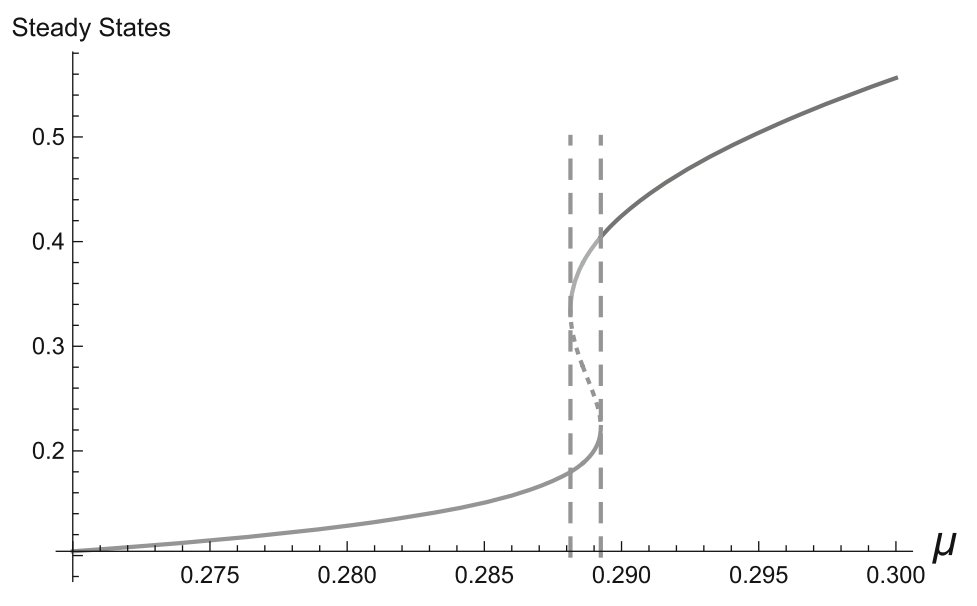
\includegraphics[width=0.8\linewidth]{Chapters/2_Ca2+_Models/extras/kaouristeadystates.PNG}
  \caption{A graph that shows the steady states of the non-dimensionalised form of the model, \eqref{origatri1stnondim}, \eqref{origatri2ndnondim}. The steady states are shown as a function of the bifurcation parameter $\mu(p)$. We can see that as $\mu(p)$ increases, there is one steady state. There is a double (degenerate) steady state at $\mu(p)=0.28814$. There are then three steady states, followed by another double (degenerate) steady state at $\mu(p)=0.28925$. Finally, there is just one steady state for all $\mu(p)>0.28925$. Source: \citeA{kaouri}.}
\end{figure}

To identify the bifurcations of the Atri model, we start by linearising the system near its
steady states. Then, for each steady state we compute the Jacobian matrix. Let
\begin{align}
    \frac{dc}{dt}&=F(c,n),\nonumber\\
    \frac{dn}{dt}&=G(c,n).\nonumber
\end{align}
The Jacobian matrix is given by
\begin{equation*}
J = 
\begin{pmatrix}
J_{1,1} & J_{1,2}\\
J_{2,1} & J_{2,2}
\end{pmatrix},
\end{equation*}
where
\begin{align}
J_{1,1}=\frac{\partial F}{\partial c}\text{,  } J_{1,2}=\frac{\partial F}{\partial n}\text{,  } J_{2,1}=\frac{\partial G}{\partial c}\text{,  } J_{2,2}=\frac{\partial G}{\partial n},\nonumber
\end{align}
are evaluated at steady-state. The characteristic polynomial of the system is given by
\begin{equation}
    \lambda^2-T(J)\lambda+D(J)=0,\nonumber
\end{equation}
where the trace, determinant and discriminant are defined respectively as follows:
\begin{align}
    T(J)=&J_{1,1}+J_{2,2},\nonumber\\
    D(J)=&J_{1,1}J_{2,2}-J_{1,2}J_{2,1},\nonumber\\
    Disc(J)=&(T(J))^2-4D(J).\nonumber
\end{align}
The trace, determinant and discriminant are important in the understanding of the qualitative behaviour of the system. Our trace and determinant are given by
\begin{align}
T(J)=&\frac{\mu (p)K_1n}{c+1}-\frac{\mu(p)K_1n(b+c)}{(c+1)^2}-\frac{V}{K+c}+\frac{Vc}{(K+c)^2}-1,\nonumber\\
D(J)=&-\frac{\mu(p)K_1n}{c+1}+\frac{\mu(p)K_1n(b+c)}{(c+1)^2}+\frac{V}{K+c}-\frac{Vc}{(K+c)^2}+\frac{2\mu(p)K_1(b+c)c}{(c+1)(c^2+1)^2},\nonumber
\end{align}
where $\lambda$ represents the eigenvalues. We can therefore solve the characteristic polynomial to find these eigenvalues. Eigenvalues, $\lambda$, are given by the following:
\begin{equation}
    \lambda = \frac{T(J) \pm \sqrt{T(J)^2-4D(J)}}{2}.\nonumber
\end{equation}
In \citeA{kaouri} is a complete list of bifurcations of the system. These are found by determining the nature of the roots of the polynomial over a range of values for $\mu(p)$. {The list of bifurcations from \citeA{kaouri} is as follows.}
\begin{itemize}
\item $0 <\mu< 0.27828$: one stable node.
\item $\mu = 0.27828$: the stable node becomes a stable spiral (bifurcation $Disc = 0$)
\item $\mu = 0.28814$: Stable spiral present. Also, a saddle and an unstable node
emerge (bifurcation $Det = 0$, {fold point})
\item $\mu = 0.28900$: the stable spiral becomes an unstable spiral. The other two steady states are still a saddle and an unstable node. ($Tr=0$, Hopf bifurcation)
\item $\mu = 0.28924$ the unstable spiral becomes an unstable node, and we have two
unstable nodes and a saddle ($Disc = 0$)
\item $\mu = 0.28925$: one unstable node ($Det = 0$, {fold point})
\item $\mu = 0.28950$: the unstable node becomes an unstable spiral ($Disc = 0$)
\item $\mu = 0.49500$: the unstable spiral becomes a stable spiral. ($Tr=0$, Hopf bifurcation)
\end{itemize}

\begin{figure}[h!!!t!!!b!!!p]
  \centering
  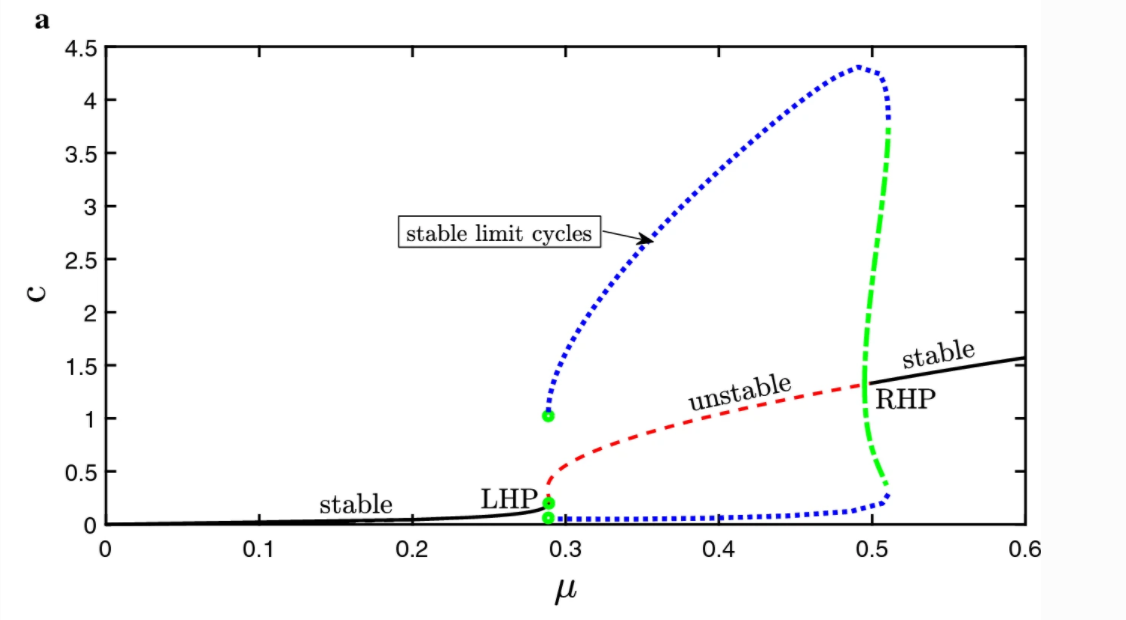
\includegraphics[width=1\linewidth]{Chapters/2_Ca2+_Models/extras/cbifmu.PNG}
  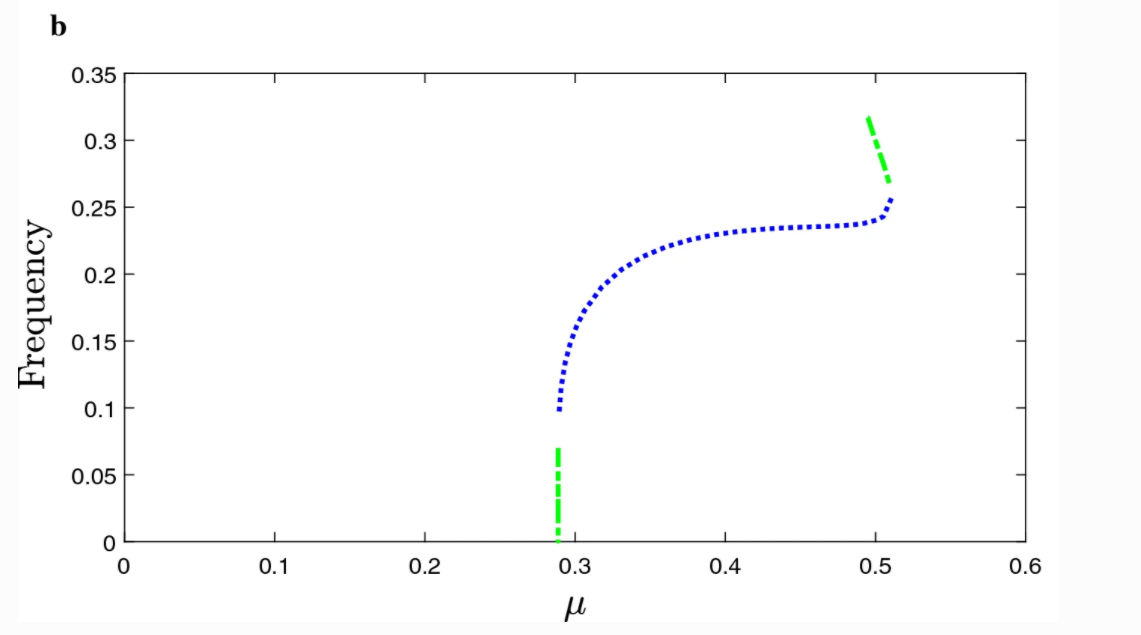
\includegraphics[width=1\linewidth]{Chapters/2_Ca2+_Models/extras/freqbigmu.PNG}
  \caption{Bifurcation diagrams for the non-dimensionalised Atri model \eqref{origatri1stnondim}, \eqref{origatri2ndnondim} as $\mu(p)$ increases. (\textbf{a}) Amplitude of calcium oscillations (limit cycles). The blue dots show the stable limit cycles while the green dashes show the unstable limit cycles. Note the presence of the left Hopf point (LHP) and the right Hopf point (RHP). {(\textbf{b}) Frequency of the limit cycles. }Source: \citeA{kaouri}. }\label{Kaouribif}
\end{figure}

\subsection{Simulations}
We now look at the simulations of the Atri model in different bifurcation regimes. We use the $ode45$ function in MATLAB \cite{MATLAB2020} to solve {the reduced }equations, \eqref{origatri1stnondim} and \eqref{origatri2ndnondim}, with various values of $\mu(p)$. Figure \ref{figorigatri} shows $Ca^{2+}$ oscillations as solutions to the Atri Model, (\ref{origatri1stnondim}), (\ref{origatri2ndnondim}), with $\mu(p)=0.3$ (within oscillatory range). Figure \ref{figmuphighlow} also shows $Ca^{2+}$ oscillations as solutions to the Atri model (\ref{origatri1stnondim}), (\ref{origatri2ndnondim}). In \textbf{A}, there is a simulation with $\mu(p)=0.2886$ (too low to be in the oscillatory range). Here, both $c$ and $n$ quickly go to their respective steady state values. In \textbf{B}, there is a simulation with $\mu(p)=0.6$ (too high to be in the oscillatory range). Oscillations start with a large amplitude and dampen over time.

\begin{figure}[h!!!t!!!b!!!p]
  \centering
  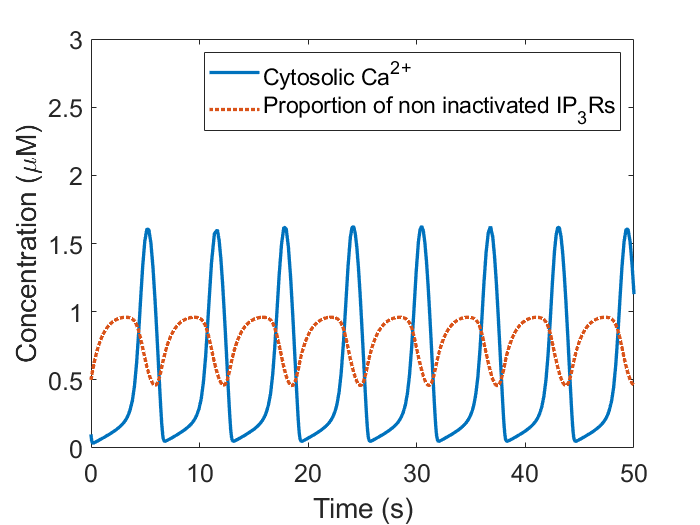
\includegraphics[width=0.6\linewidth]{Chapters/2_Ca2+_Models/extras/orginalatrimu1.png}
  \caption{$Ca^{2+}$ oscillations as solutions to the Atri Model, (\ref{origatri1stnondim}), (\ref{origatri2ndnondim}), with $\mu(p)=0.3$ (within oscillatory range). Parameter values are shown in Table \ref{origatriparam}. Initial values of $0.1\mu M$ and $0.5$ were taken for $c$ and $n$ respectively. Oscillations over time of $50$ seconds. \textit{Software:} MATLAB.}\label{figorigatri}
\end{figure}

\begin{figure}[!htbp]
\centering
\minipage{0.6\textwidth}
  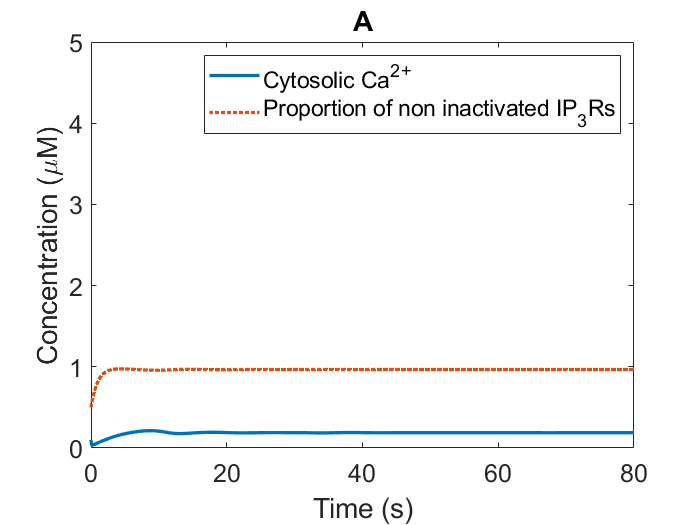
\includegraphics[width=\linewidth]{Chapters/2_Ca2+_Models/extras/originalatrimu0.5.png}
\endminipage\hfill\\
\minipage{0.6\textwidth}
  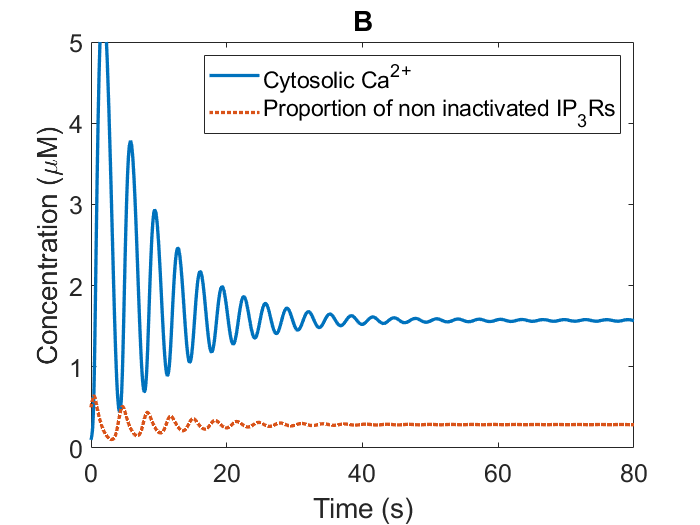
\includegraphics[width=\linewidth]{Chapters/2_Ca2+_Models/extras/originalatri1.5.png}
\endminipage\hfill
\caption{$Ca^{2+}$ oscillations as solutions to the Atri model (\ref{origatri1stnondim}), (\ref{origatri2ndnondim}). Parameter values are shown in Table \ref{origatriparam}. Initial values of $0.1$ and $0.5$ were taken for $c$ and $n$, respectively. (\textbf{A}) Simulation with $\mu(p)=0.2886$ (too low to be within oscillatory range). Here, both $c$ and $n$ quickly go to their respective steady state values. (\textbf{B}) Simulation with $\mu(p)=0.6$ (too high to be within oscillatory range). Oscillations start with a large amplitude and dampen over time. \textit{Software:} MATLAB.}\label{figmuphighlow}
\end{figure}

\subsubsection{Bifurcation diagram}
Non-dimensionalisation has reduced the number of parameters in the system. Equations (\ref{origatri1stnondim}) and (\ref{origatri2ndnondim}) can be used to generate a bifurcation diagram for $\mu(p)$ against $c$. Figure \ref{Kaouribif} \cite{kaouri} shows the changes in the qualitative behaviour of the system as $\mu(p)$ increases, generated with the XPPAUT continuation software \cite{xppaut}. They show the amplitude and frequency of limit cycles, respectively, as the bifurcation parameter $\mu(p)$ increases. In Figure \ref{Kaouribif}\textbf{a} we see for what values of $\mu(p)$ we have stable and unstable limit cycles, and the two Hopf points. The figures show that as $\mu(p)$ is increased, oscillations increase more in amplitude than they do in frequency. The range of $\mu (p)$ that gives oscillations is $0.289<\mu <0.495$.

We have now presented in detail the \citeA{atri} model and its derivation, linear stability analysis and bifurcation analysis. This model captures key $Ca^{2+}$ signalling features but uses outdated data to model the $IP_3R$ dynamics. More recent experiments and data have shown that the probabilities $p_1$, $p_2$, and $p_3$ are more accurately modelled by \citeA{Mak1998}. We will incorporate the latter $IP_3R$ dynamics in a model later in the thesis.

Next, we present in detail the Li-Rinzel model and we compare it to the Atri model.

\section{The Li-Rinzel model}
The \citeA{lirinzel} model shares many key features with the Atri model. It is also a two--variable gating model obtained by reducing the 9--variable \citeA{deyoungkeizer} model for $Ca^{2+}$ oscillations mediated by $IP_3R$. It is based on the assumption of there being three binding sites for the $IP_3R$ - those are the sites responsible for $IP_3$ regulation, $Ca^{2+}$ activation and $Ca^{2+}$ inactivation. The Li-Rinzel model has a bifurcation diagram almost identical to that of the De Young-Keizer model, and is analogous in its form to the Hodgkin-Huxley equations \cite{hodgkinhuxley}, a gating model for plasma membrane electrical excitability. The bifurcation diagram for the Li-Rinzel model also compares closely to the bifurcation diagram of the Atri model. The Li-Rinzel model retains the most important dynamic features of the De Young-Keizer model and is able to reproduce experimental observations \shortcite{Bezprovannywatras, watras1991}. The two--variable Li-Rinzel model is as follows:
\begin{align}
    \frac{dc}{dt}=&\left(v_1\left(\frac{p}{p+K_{IP_3}}\right)^3\left(\frac{c}{c+K_{act}}\right)^3n^3+\epsilon\right)(c_0-(1+c_1)c)-\frac{V_ec^2}{K_e^2+c^2}\label{lirinzeltwovar1},\\
    \frac{dn}{dt}=&A(c+K_{inh})\left(\frac{K_{inh}}{c+K_{inh}}-n\right),\label{lirinzeltwovar2}
\end{align}

where $c$ is the cytosolic $Ca^{2+}$ concentration and $n$ is the proportion of non inactivated $IP_3R$. The maximal rate of $Ca^{2+}$ release is given by $v_1$. The half-activation constant for $IP_3$ binding to activation site 1 is given by $K_{IP_3}$. {In all cells, there are SERCA pumps on the ER which allow $Ca^{2+}$ to be pumped back into the ER. Here, this flux is assumed to be governed by a Hill function which saturates for a sufficiently high value of $Ca^{2+}$.} The maximal SERCA pump rate is given by $V_e$, and the half-activation constant for the SERCA pumps is $K_e$. A parameter to characterize the slow time scale of $Ca^{2+}$ inactivation is given by $A$. The half-maximal inactivation constant for $Ca^{2+}$ binding to the inhibitory site 3 is $K_{inh}$. Finally, $\epsilon$ represents the $Ca^{2+}$ leak out of the ER.

\subsubsection*{Model assumptions}
The $Ca^{2+}$ permeability of the $IP_3R$ is its maximum permeability times the channels open probability. The Li-Rinzel model \eqref{lirinzeltwovar1}, \eqref{lirinzeltwovar2}, is built on assuming the existence of three binding sites on each subunit of the channel. Similarly to the model assumptions for the Atri model, we have the sites for:
\begin{itemize}
\item A single molecule of $IP_3$ binds to the $IP_3$ activation site (site 1).
\item A single molecule of $Ca^{2+}$ binds to the $Ca^{2+}$ activation site (site 2).
\item Two molecules of $Ca^{2+}$ bind to the $Ca^{2+}$ inhibitory site (site 3).
\end{itemize}

These three binding processes are not necessarily assumed to be independent. Firstly, $IP_3$ binding depends on whether the $Ca^{2+}$ inhibitory site is occupied, while $Ca^{2+}$ binding to its inhibitory site also depends on whether the receptor already has an $IP_3$ molecule bound. However, these two processes are independent of $Ca^{2+}$ binding to its activation site. This independence gives rise to some symmetries in the binding rate constants. For generality, we assume that three binding processes depend on each other, with no symmetry assumed.

The channel's open probability at equilibrium is expressed as
\begin{equation}
    \left(\frac{p}{p+K_{IP_3}}\right)^3\left(\frac{c}{c+K_{act}}\right)^3\left(\frac{K_{inh}}{K_{inh}+c}\right)^3.
\end{equation}
This fits to experimental data of the bell-shaped $Ca^{2+}$ dependence and the sigmoidal $IP_3$ dependence of the $IP_3R$ open probability at equilibrium \shortcite{Bezprovannywatras, deyoungkeizer}.

\subsubsection*{Dynamic behaviour of the $\mathbf{IP_3R}$}
The De Young-Keizer model {was reduced} to the two--variable Li-Rinzel model. As a consequence of time scale separation, it turns out that the effect of specific gating processes are independent of the kinetics of a slower gating process but dependent on all faster gating processes. This means that the channel opening by $IP_3$ seems to be independent of $Ca^{2+}$ binding to either the activation or inhibitory site since it is faster than those processes. 

The Li-Rinzel model can be compared to the Atri model. They hold many similarities and are still widely used by modellers today. The equation for $n$ is almost identical in the Atri model and the Li-Rinzel model. The equations for $c$ hold very similar structures in both of these models. Equation \eqref{lirinzeltwovar1} represents cytosolic $Ca^{2+}$ concentration ($\mu M$) and can be compared to equation \eqref{origatri1st} from the Atri model. Equation \eqref{lirinzeltwovar2} represents the proportion of non inactivated $IP_3R$ and can be compared to equation \eqref{origatri2nd}. Like equation \eqref{origatri1st}, equation \eqref{lirinzeltwovar1} has a positive term for $Ca^{2+}$ flux into the cytosol, with Hill functions of order 1. We can compare $p_1$, $p_2$, $p_3$ from the Atri model to the equivalent terms here. The probability of $IP_3$ binding to its activation site is represented again by a Hill equation, $p/(p+K_{IP_3})$. This implies that no $IP_3R$ are activated when there is no $IP_3$ present, or in other words the open probability of the $IP_3R$ is $0$. The term here corresponds to $p_1$ in the Atri model. The probability of $Ca^{2+}$ binding to its activation site is represented by $c/(c+K_{act})$. This term corresponds to $p_2$ in the Atri model. Finally, the probability that $Ca^{2+}$ is not bound to its inhibitory site is represented by $K_{inh}/(K_{inh}+c)$. This is a Hill function of order 1, in comparison to $p_3$ in the Atri model being a Hill function of order 2. The three terms for probabilities $p_1$, $p_2$ and $p_3$ are raised to the third power in the Li-Rinzel model. As discussed, these probabilities are all modelled by Hill functions. The simplified equation is analogous, mathematically, to the \citeA{hodgkinhuxley} model of plasma membrane electrical excitability. {In the Li-Rinzel model, $c$ (analogous to the membrane voltage) is the major regulator of the $IP_3R$ and the concentration gradient $c-c_0$ (analogous to the voltage deviation from the Nernst reversal potential) is the driving force for oscillations. In both models, channel activation and inactivation appear as separate factors with first-order gating kinetics.} There is also a negative term in equation \eqref{lirinzeltwovar1} representing $Ca^{2+}$ being pumped back into the ER. This term for the SERCA pumps is a Hill function of order 2. This is similar to what we have in the Atri model in equation \eqref{origatri1st}.

\subsection{Simulations}
In Figure \ref{lirinzelbif} we present the bifurcation diagram from the Li-Rinzel model \eqref{lirinzeltwovar1}-\eqref{lirinzeltwovar2}. This bifurcation diagram shows good agreement between the Li-Rinzel model and the De Young-Keizer model. The reduction from nine to two variables is therefore appropriate. {The reduction in the number of variables is useful because the model can then be very quickly studied and intuition about the system dynamics can be extracted easily}.

\begin{figure}[h!!!t!!!b!!!p]
  \centering
  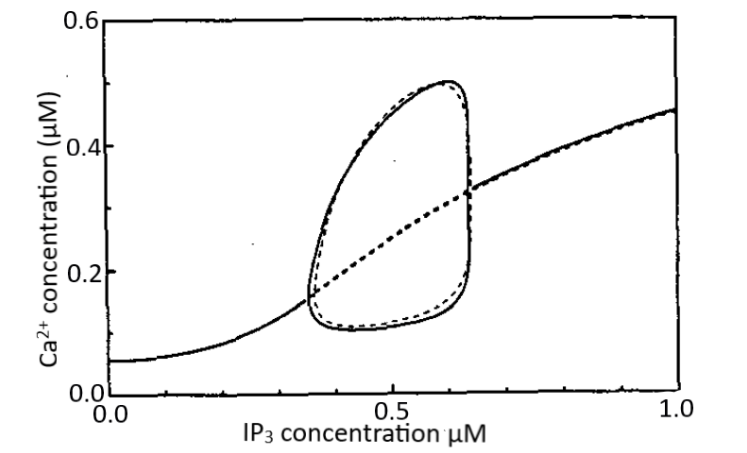
\includegraphics[width=0.8\linewidth]{Chapters/2_Ca2+_Models/extras/lirinzelbif.png}
  \caption{Bifurcation diagram with bifurcation parameter $p$ for the Li-Rinzel model, \eqref{lirinzeltwovar1}-\eqref{lirinzeltwovar2}. Source: \citeA{lirinzel}. }\label{lirinzelbif}
\end{figure}

Presented in Figure \ref{twovarminmodel} are the $Ca^{2+}$ oscillations arising as solutions to the Li-Rinzel model \eqref{lirinzeltwovar1}-\eqref{lirinzeltwovar2}. These oscillations occur with $IP_3$ concentration at $0.6 \mu M$. Parameter values are given in Table \ref{twovarminmodelparam}. There is a range of concentration for $IP_3$ for which we obtain oscillations. Shown in Figure \ref{twovarlowhigh} are graphs where the $IP_3$ concentration is too low ($0.2 \mu M$) to obtain oscillations, and too high to obtain oscillations ($1 \mu M$), respectively. {When $[IP_3]<0.47325 \mu M$,} the solution reaches steady state. Where the $IP_3$ concentration is too high, the solution decays to the steady state in an oscillatory manner. 

\begin{figure}[h!!!t!!!b!!!p]
  \centering
  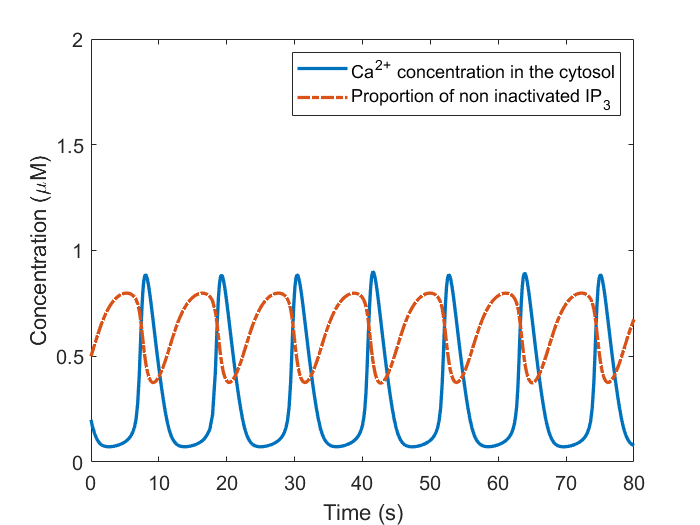
\includegraphics[width=0.7\linewidth]{Chapters/2_Ca2+_Models/extras/twovarmminimalmodel.png}
  \caption{Cytosolic $Ca^{2+}$ oscillations arising as solutions to the Li-Rinzel model, (\ref{lirinzeltwovar1}), (\ref{lirinzeltwovar2}). Parameter values used are in Table \ref{twovarminmodel}. To be within oscillatory range, the $IP_3$ level, $p$, was chosen to be $0.6 \mu M$. Initial conditions applied were $0.2\mu M$ and $0.5 \mu M$ for cytosolic $Ca^{2+}$ and for the proportion of non inactivated $IP_3R$, respectively. \textit{Software:} MATLAB. }\label{twovarminmodel}
\end{figure}

\begin{figure}[!htb]
\centering
\minipage{0.6\textwidth}
  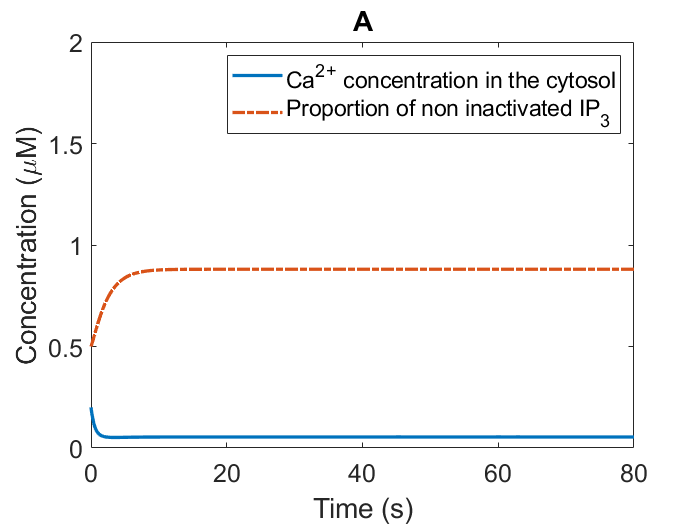
\includegraphics[width=\linewidth]{Chapters/2_Ca2+_Models/extras/twovarlow.png}
\endminipage\hfill\\
\minipage{0.6\textwidth}
  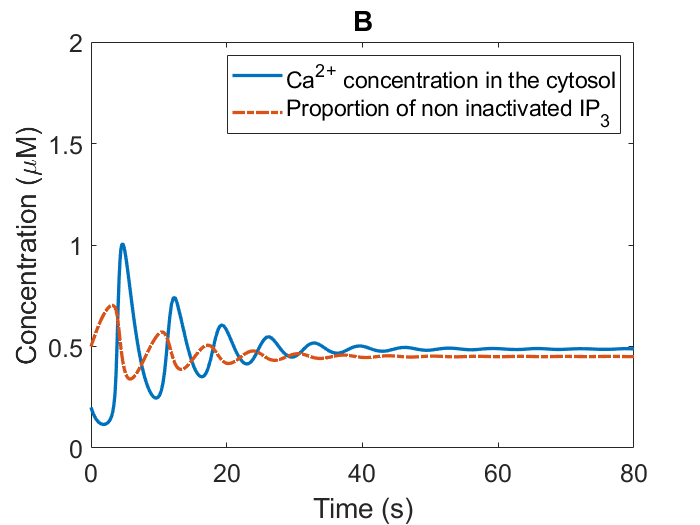
\includegraphics[width=\linewidth]{Chapters/2_Ca2+_Models/extras/twovarhigh.png}
\endminipage\hfill
\caption{Decaying $Ca^{2+}$ oscillations arising as solutions to the two--variable minimal model by \citeA{lirinzel}, (\ref{lirinzeltwovar1})-(\ref{lirinzeltwovar2}). Parameter values used are shown in Table \ref{twovarminmodel}. Initial conditions applied were $0.2\mu M$ and $0.5$ for cytosolic $Ca^{2+}$ and the proportion of non inactivated $IP_3R$ respectively. (\textbf{A}) $IP_3=0.2\mu M$, too low to be within oscillatory range. (\textbf{B}) $IP_3=1\mu M$, too high to be within oscillatory range. \textit{Software:} MATLAB.}\label{twovarlowhigh}
\end{figure}

We have now studied two famous gating models - the Atri model and the Li-Rinzel model. As discussed in the Introduction, many modellers have built on these two--variable models to derive more complex $Ca^{2+}$ signalling models. Having studied the $IP_3R$ dynamics in these models, in the next chapter we go on to review more up-to-date data of these dynamics from experiments carried out by \citeA{Mak1998}, and how these data were fitted to an equation for the open probability of the $IP_3R$. Our aim is to eventually find a way to incorporate these more detailed and exact $IP_3R$ dynamics into a model for $Ca^{2+}$ signalling in fertilising eggs. 
